\begin{figure}
\begin{tabular}{@{}c@{}c@{}}
\begin{subfigure}[b]{0.43\textwidth}
\begin{center}
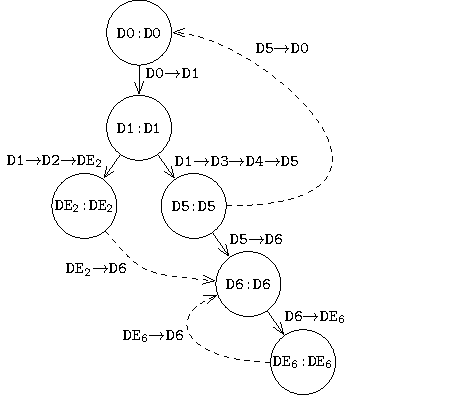
\includegraphics[scale=1]{chapters/figures/figClistDeconsProductCfg.pdf}
\end{center}
\caption{\label{fig:clistdeconsproductcfg}Decons-PCFG}
\end{subfigure}%
&
\begin{subfigure}[b]{0.54\textwidth}
\begin{center}
\begin{footnotesize}
\renewcommand{\arraystretch}{1.3}
\begin{tabular}{cl}
\toprule
{\bf PC-Pair} & \multicolumn{1}{c}{\bf Invariants} \\
\toprule
(\ddpc{0}{0}) & \Tstrut $\circled{\small P} \  \fstv{l} = \sndv{l}$ \\
\midrule
(\ddpc{1}{1}) & \Tstrut $\circled{I1} \  \fstv{l} = \sndv{l}$ \\
\midrule
\multirow{2}{*}{(\ddpc{5}{5})} &
\Tstrut $\circled{I2} \  \fstv{val} = \sndv{val}$ \\
& \Bstrut $\circled{I3} \  \structPointer{\fstv{l}}{\mem{}}{lnode}{next} = \structPointer{\sndv{l}}{\mem{}'}{lnode}{next}$ \\
\midrule
\multirow{2}{*}{(\ddpc{6}{6})} &
\Tstrut $\circled{I4} \  \fstv{val} = \sndv{val}$ \\
& \Tstrut \Bstrut $\circled{I5} \  \fstv{tail} = \sndv{tail}$ \\
\midrule
\Tstrut (\ddpc{E_2}{E_2}) &
\multirow{2}{*}{$\circled{E} \   \fstv{ret} = \sndv{ret}$} \\
\Bstrut (\ddpc{E_6}{E_6}) & \\
\bottomrule
\end{tabular}
\end{footnotesize}
\end{center}
\caption{\label{fig:clistdeconsproductcfginvs}Node invariants for decons-PCFG in \cref{fig:clistdeconsproductcfg}}
\end{subfigure}%
\\
\end{tabular}
\caption{\label{fig:clistdeconsproductcfgandinvs}Decons-PCFG and its associated node invariants for the deconstruction programs based on \lifted{list}{\mem{}}{lnode}{\cv{l}} and \lifted{list}{\mem{}'}{lnode}{\cv{l}} respectively.}
\end{figure}